\documentclass{standalone}
\usepackage{tikz}
\usetikzlibrary{decorations.pathreplacing}
\usepackage{amsfonts}


\begin{document}
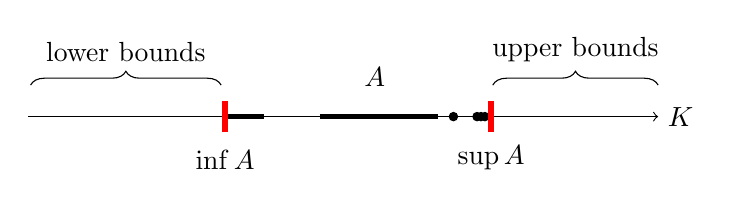
\begin{tikzpicture}
% Draw the real line
  \draw[->] (-4,0) -- (4,0) node[right] {$K$};
  
  % Draw the point 'x' and '0'

 
  \draw[black, line width=2pt] (-1.5,0) -- (-1,0);
    \draw[black, line width=2pt] (-0.3,0) -- (1.2,0);

  \filldraw (1.4,0) circle (1.5pt);
  
  \filldraw (1.7,0) circle (1.5pt);
  \filldraw (1.75,0) circle (1.5pt);
  \filldraw (1.8,0) circle (1.5pt);

  
  \node at (0.4, 0.5) {$A$};
  
  % Draw the brace and label it
  \draw[decorate,decoration={brace,amplitude=5pt}] (-3.97,0.4) -- (-1.55,0.4) node[midway,above=5pt] {\mbox{lower bounds}};
  
  \draw[line width=2pt, red] (-1.5,-0.2) -- (-1.5,0.2);
  \node[anchor=south] at (-1.5,-0.8) {$\inf A$};
  
  
   \draw[decorate,decoration={brace,amplitude=5pt}] (1.9,0.4) -- (4,0.4) node[midway,above=5pt] {\mbox{upper bounds}};
  
  \draw[line width=2pt, red] (1.88,-0.2) -- (1.88,0.2);
  \node[anchor=south] at (1.88,-0.8) {$\sup A$};
  

  
  
  
  \end{tikzpicture}
\end{document}